\section{Intensity Transformation and Spatial Filtering}
\subsection{Histogram Equalization}
Das Ziel ist es, ein Bild mit einer Normalverteilung zu erhalten (Histogram Flach und Fläche $1$), damit der dynamische Bereich gut genutzt wird. Weil beim Histogram die Punkte gerundet werden müssen, sind absolut Flache Histogramme sehr selten.

\[
s = T(r) = (L-1)\int_{0}^{r}p_r(\omega)d\omega
\]

\subsection{Histogram Matching}
\[
z = G^{-1}\left[T(r)\right] = G^{-1}(s)
\]

\subsection{Bild Erweiterung}
Durchschnitt
\[
m = \sum_{i=0}^{L-1}r_ip(r_i)
\]
n-th Bewegung ($\mu_2 = \sigma^2$)
\[
\mu_n(r) = \sum_{i=0}^{L-1}(r_i - m^n)p(r_i)
\]
Sample Schnitt
\[
m = \frac{1}{MN}\sum_{x=0}^{M-1}\sum_{y=0}^{N-1}f(x,y)
\]
Sample Varianz
\[
\sigma^2 = \frac{1}{MN}\sum_{x=0}^{M-1}\sum_{y=0}^{N-1}[f(x,y) -m]^2
\]

\textbf{Beispiel}: $5\times5$ Bild mit $L=4$, weil Werte von $0..3$ gehen:
\begin{center}
	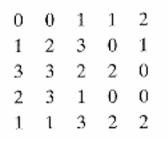
\includegraphics[width=0.2\columnwidth]{Images/histo_ex}
\end{center}
\[
p(r_0) = \frac{6}{25};\quad p(r_1)  = \frac{7}{25};\quad p(r_2) = \frac{7}{25};\quad p(r_3) = \frac{5}{25}
\]

\[
m = \sum_{i=0}^{3}r_ip(r_i) = (0)(\frac{6}{25}) + \dots + (3)(\frac{5}{25}) = 1.44
\]

\subsection{Spatial Filtering}
Correlation schiebt den Filter über den Eingang und berechnet die Summe an jedem Punkt. Convolution macht das selbe, jedoch wird der Filter gedreht um (Oben/unten) \underline{UND} (Links/Rechts)
\begin{center}
	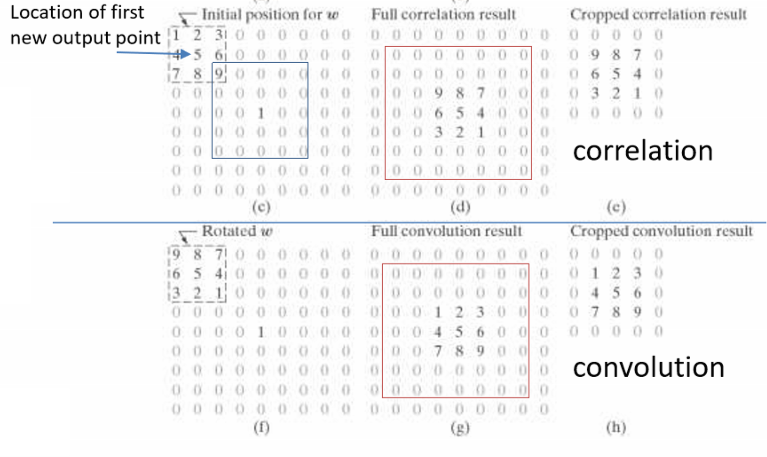
\includegraphics[width=\columnwidth]{Images/conv_cor}
\end{center}

\textbf{Beispiel}
\begin{center}
	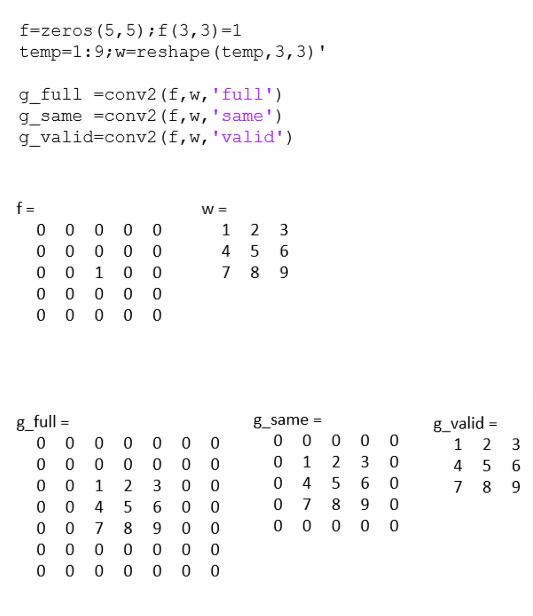
\includegraphics[width=\columnwidth]{Images/conv_cor_m}
\end{center}

